\chapter{Handbook}
 
\section{Chapters}

\section{Paragraphs}

\section{Citation}

\section{Font Format}
 
Some of the \textbf{greatest} discoveries in \underline{science} were made by \textbf{\textit{accident}}. This is an \emph{emphasized} word inside normal text. \textit{And this is an \emph{emphasized} word inside an italicized text.}

\subsection{Bold}
\begin{lstlisting}
  \textbf{<your text>}
\end{lstlisting}

\subsection{Underline}
\begin{lstlisting}
  \underline{<your text>}
\end{lstlisting}

\subsection{Italic}
\begin{lstlisting}
  \textit{<your text>}
\end{lstlisting}

\subsection{Emphasis}
\begin{lstlisting}
  \emph{<your text>}
\end{lstlisting}
 
\section{Images and Figures}

\subsection{Baseline images}

Lorem ipsum dolor sit amet, consectetur adipiscing elit. Suspendisse nec pellentesque nunc. Sed massa diam, gravida ut est sit amet, molestie viverra nunc. Nam id ex ut tortor viverra auctor. 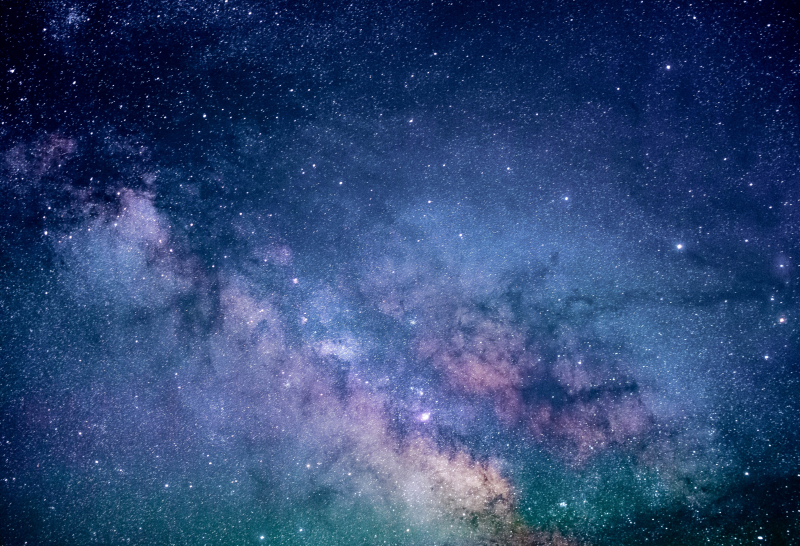
\includegraphics[height=\baselineskip]{image-1} Lorem ipsum dolor sit amet, consectetur adipiscing elit. Suspendisse nec pellentesque nunc. Sed massa diam, gravida ut est sit amet, molestie viverra nunc. Nam id ex ut tortor viverra auctor. 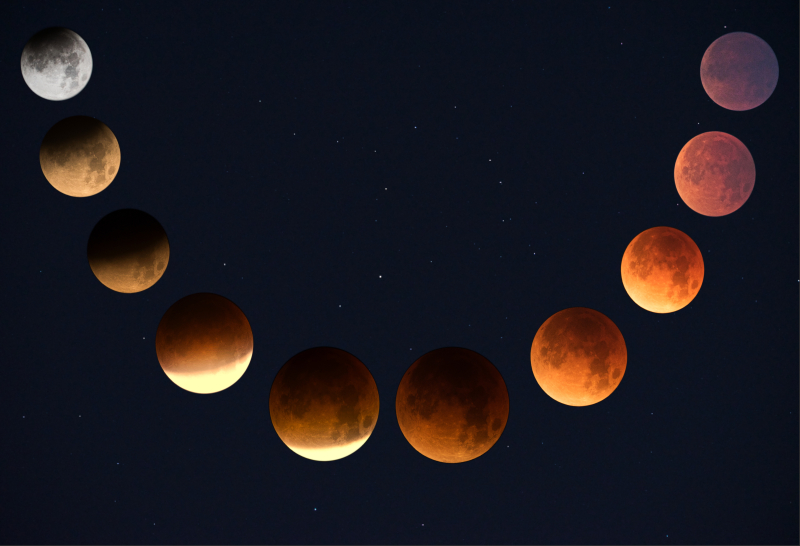
\includegraphics[height=\baselineskip]{image-2}.

\begin{lstlisting}
  \includegraphics[height=\baselineskip]{<file-name>}
\end{lstlisting}

\clearpage
\subsection{Full width image}

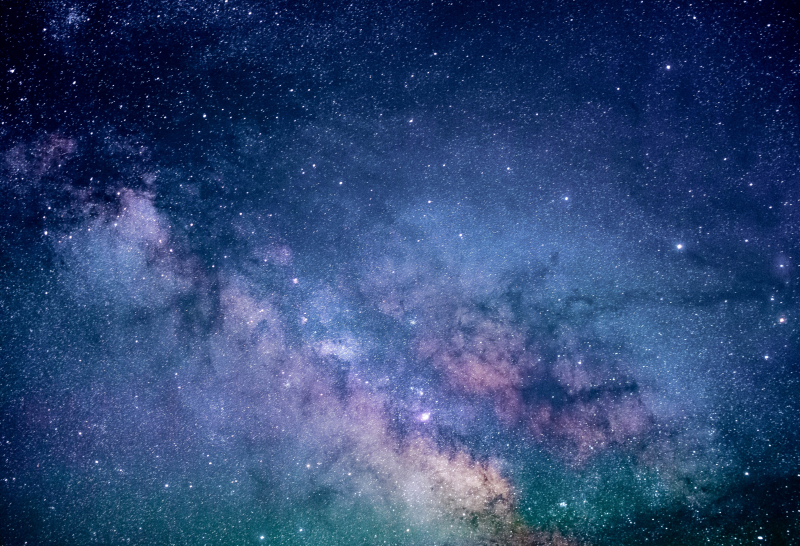
\includegraphics[width=\linewidth]{image-1}

\begin{lstlisting}
  \includegraphics[width=\linewidth]{<file-name>}
\end{lstlisting}

\clearpage
\subsection{Image with specific height}

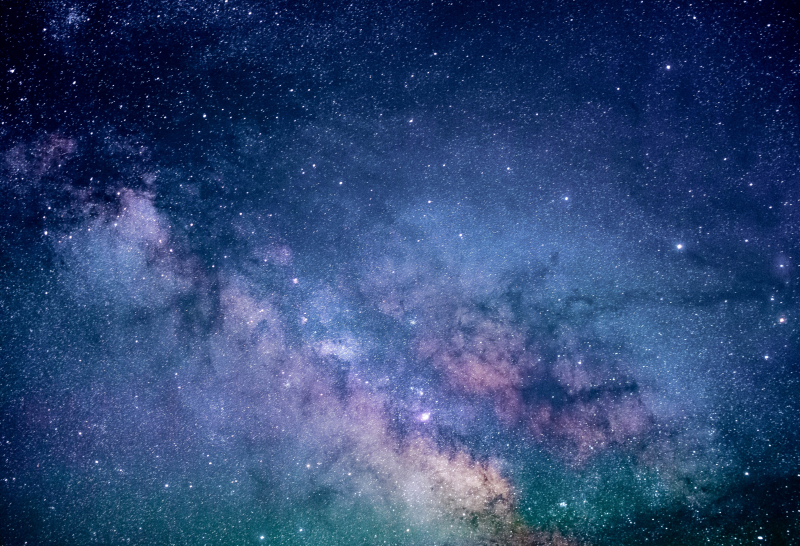
\includegraphics[height=3cm]{image-1}

\begin{lstlisting}
  \includegraphics[height=3cm]{<file-name>}
\end{lstlisting}

\clearpage
\subsection{Grid of images}

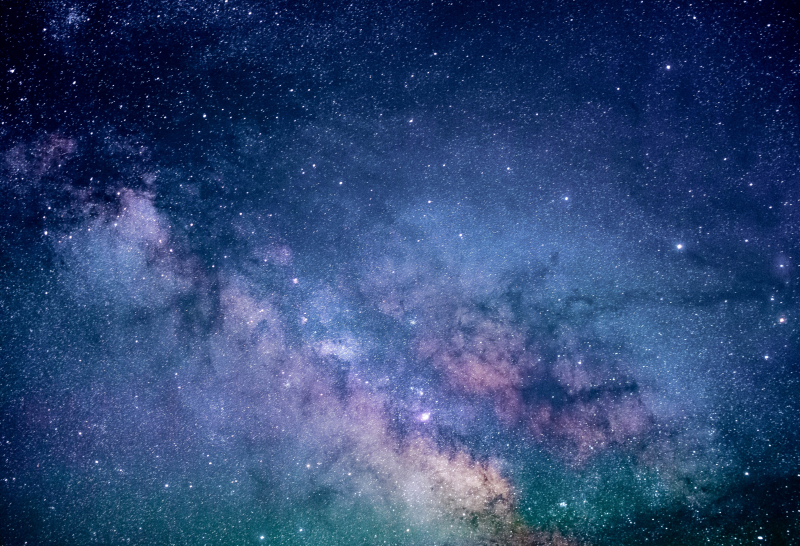
\includegraphics[width=0.3\linewidth]{image-1}
\quad
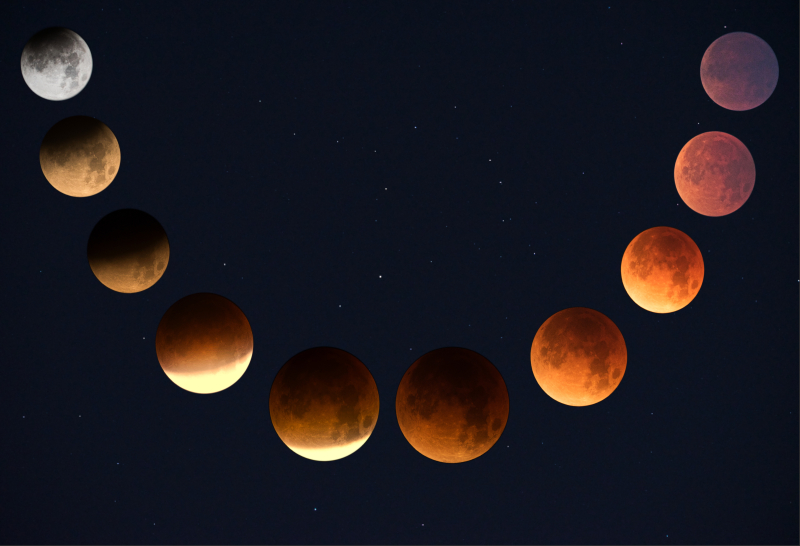
\includegraphics[width=0.3\linewidth]{image-2}
\quad
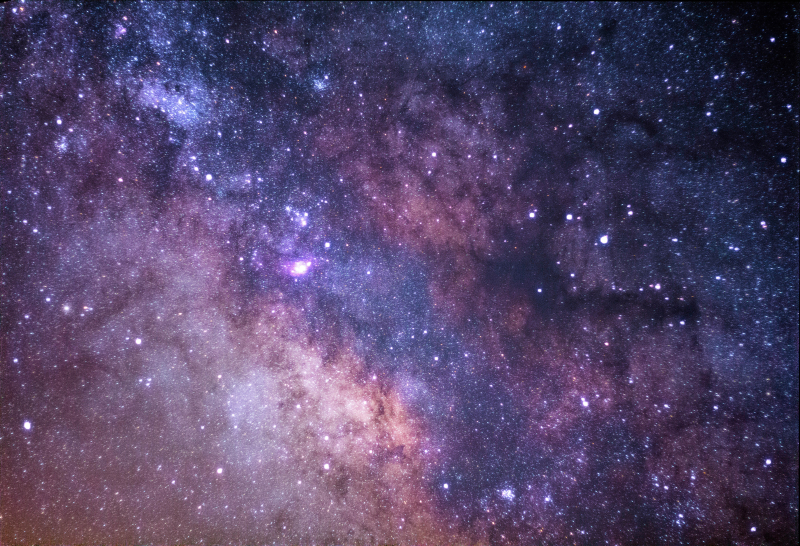
\includegraphics[width=0.3\linewidth]{image-3}
\\[\baselineskip]% adds vertical line spacing
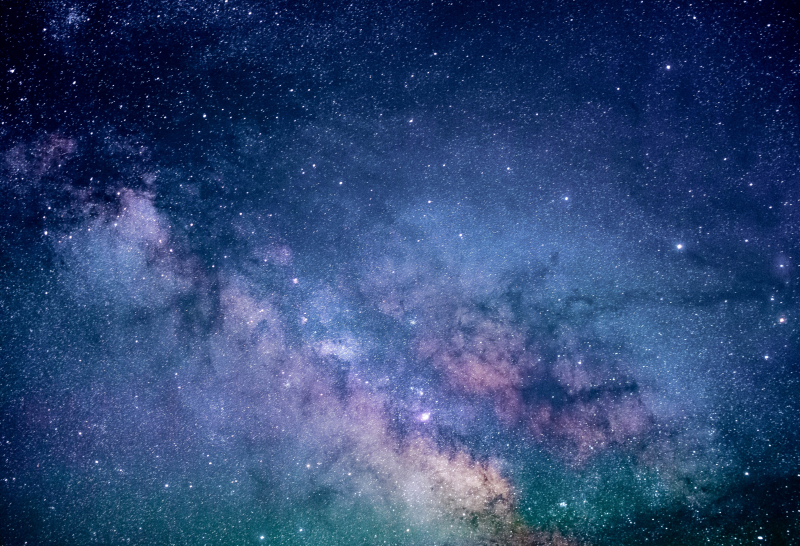
\includegraphics[width=0.3\linewidth]{image-1}
\quad
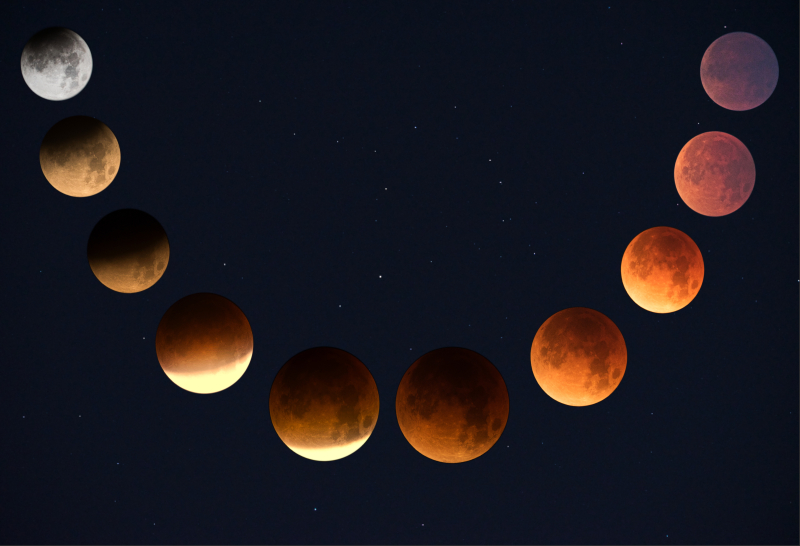
\includegraphics[width=0.3\linewidth]{image-2}
\quad
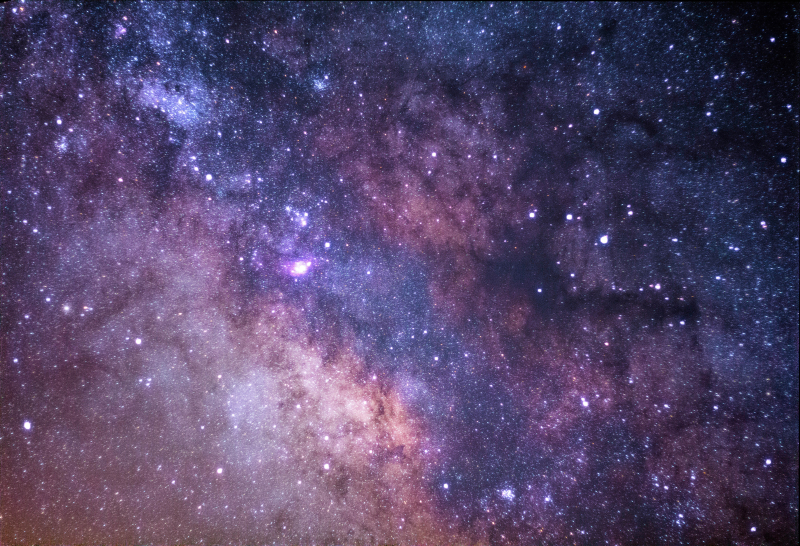
\includegraphics[width=0.3\linewidth]{image-3}

\begin{lstlisting}
  % first column
  \includegraphics[width=0.3\linewidth]{<file-name>}
  \quad % adds horizontal line spacing
  \includegraphics[width=0.3\linewidth]{<file-name>}
  \quad
  \includegraphics[width=0.3\linewidth]{<file-name>}

  \\[\baselineskip] % adds vertical line spacing

  % second column
  \includegraphics[width=0.3\linewidth]{<file-name>}
  \quad
  \includegraphics[width=0.3\linewidth]{<file-name>}
  \quad
  \includegraphics[width=0.3\linewidth]{<file-name>}
\end{lstlisting}

\clearpage
\subsection{Centered Figure}

\begin{figure}[h]
  \centering
  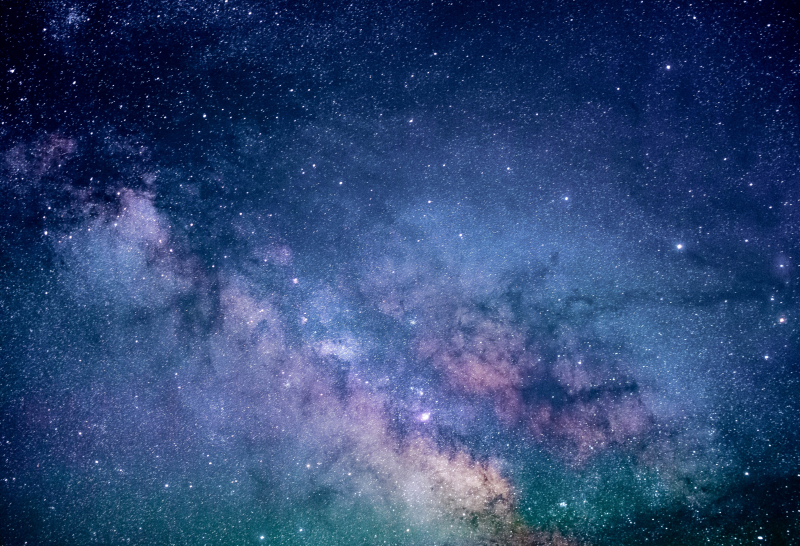
\includegraphics[width=0.5\textwidth]{image-1}
  \caption{This is a centered figure}
  \label{fig:image1}
\end{figure}

\begin{lstlisting}
  \begin{figure}[h]
    \centering
    \includegraphics[width=0.5\textwidth]{<file-name>}
    \caption{This is a centered figure}
    \label{fig:<yourFigureLabel>}
  \end{figure}
\end{lstlisting}

\clearpage
\subsection{Grid of figures}

\begin{figure}[h]
  \centering
  \begin{subfigure}{0.45\textwidth}
    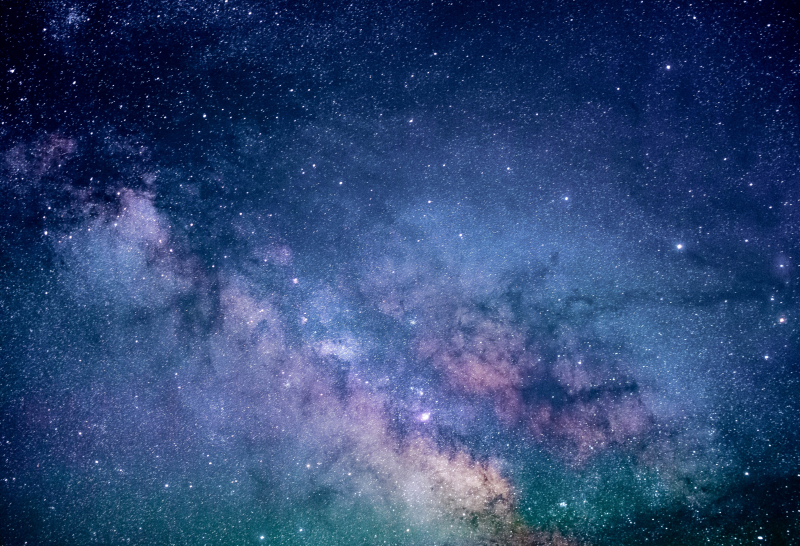
\includegraphics[width=\linewidth]{image-1} 
    \caption{Caption subfigure 1}
    \label{fig:subim1}
  \end{subfigure}%
  \quad
  \begin{subfigure}{0.45\textwidth}
    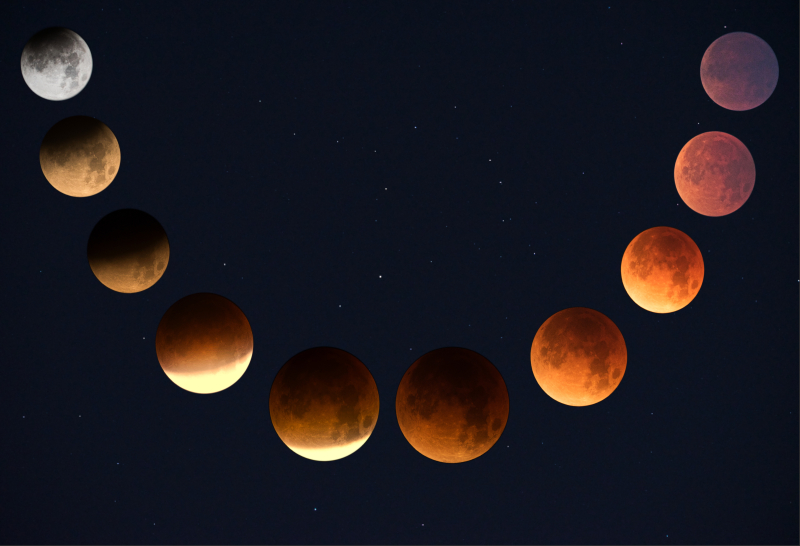
\includegraphics[width=\linewidth]{image-2}
    \caption{Caption subfigure 2}
    \label{fig:subim2}
  \end{subfigure}%
  \caption{This is a grid of figures with two images}
  \label{fig:image2}
\end{figure}

\begin{lstlisting}
  \begin{figure}[h]
    \centering
    \begin{subfigure}{0.45\textwidth}
      \includegraphics[width=\linewidth]{<file-name>} 
      \caption{Caption subfigure 1}
      \label{fig:<yourSubigureLabel>}
    \end{subfigure}%
    \quad
    \begin{subfigure}{0.45\textwidth}
      \includegraphics[width=\linewidth]{<file-name>}
      \caption{Caption subfigure 2}
      \label{fig:<yourSubigureLabel>}
    \end{subfigure}%
    \caption{This is a grid of figures with two images}
    \label{fig:<yourFigureLabel>}
  \end{figure}
\end{lstlisting}